\documentclass[11pt]{article}
\usepackage{fullpage}
\usepackage{fancyhdr}

\usepackage{amsmath}
\usepackage{amssymb}
\usepackage{url}

\usepackage{listings}
\usepackage{color}
\lstset{language=Python,
        basicstyle=\footnotesize\ttfamily,
        showspaces=false,
        showstringspaces=false,
        tabsize=2,
        breaklines=false,
        breakatwhitespace=true,
        identifierstyle=\ttfamily,
        keywordstyle=\color[rgb]{0,0,1},
        commentstyle=\color[rgb]{0.133,0.545,0.133},
        stringstyle=\color[rgb]{0.627,0.126,0.941},
    }

\usepackage[pdftex]{graphicx}

% header
\fancyhead{}
\fancyfoot{}
\fancyfoot[C]{\thepage}
\fancyhead[R]{Daniel Foreman-Mackey}
\fancyhead[L]{Statistical Natural Language Processing --- Homework 2}
\pagestyle{fancy}
\setlength{\headsep}{10pt}
\setlength{\headheight}{20pt}

% shortcuts
\newcommand{\Eq}[1]{Equation (\ref{eq:#1})}
\newcommand{\eq}[1]{Equation (\ref{eq:#1})}
\newcommand{\eqlabel}[1]{\label{eq:#1}}
\newcommand{\Fig}[1]{Figure~\ref{fig:#1}}
\newcommand{\fig}[1]{Figure~\ref{fig:#1}}
\newcommand{\figlabel}[1]{\label{fig:#1}}

\newcommand{\pr}[1]{\ensuremath{p\left (#1 \right )}}
\newcommand{\lk}[1]{\ensuremath{\mathcal{L} \left ( #1 \right )}}
\newcommand{\bvec}[1]{\ensuremath{\boldsymbol{#1}}}
\newcommand{\dd}{\ensuremath{\, \mathrm{d}}}
\newcommand{\normal}[2]{\ensuremath{\mathcal{N} \left ( #1; #2 \right ) }}
\newcommand{\T}{^\mathrm{T}}

\newcommand{\data}{\mathcal{D}}
\newcommand{\code}[1]{{\sffamily #1}}


\begin{document}

The goal of this project is to classify a noun into one of five categories
(\code{place}, \code{movie}, \code{drug}, \code{person}, or \code{company})
using only the word itself.
I'll focus on building a discriminative model based on logistic regression.

\section{A note about implementation}

Instead of using the provided Java code, I decided to implement my assignment
in Python and C.
The data manipulation and feature extraction is all performed in Python using
the standard library.
Once the feature vectors have been built, they are passed to the C code that
does the computationally heavy lifting.
The standard Python implementation of \code{BFGS} was not efficient enough for
the purposes of this assignment so I used the \code{libLBFGS}%
\footnote{\url{http://www.chokkan.org/software/liblbfgs/}} C implementation
of the \code{L-BFGS} algorithm.
All of the code used in this assignment is available on GitHub at:
\url{https://github.com/dfm/stat-nlp-nyu}.

\section{General description of logistic model}

The basic model that I'm going to focus on is a discriminative logistic
classifier.
This model has the form
\begin{eqnarray}
p(y_i\,|\,\bvec{x}_i,\,\bvec{w}) &=&
\frac{\exp\left[\bvec{w}_{y_i}\T\cdot\bvec{f}(\bvec{x}_i)\right]}
{\sum_{y^\prime}
\exp\left[\bvec{w}_{y^\prime}\T\cdot\bvec{f}(\bvec{x}_i)\right)]}
\end{eqnarray}
where $\bvec{w}_{y_i}$ is the weight vector for class $y_i$ and $\bvec{f}$ is
an operator on the word $\bvec{x}_i$ that extracts a feature vector (the same
length as $\bvec{w}_y$) describing the ``important'' characteristics of the
word.
The choice of $\bvec{f}$ proves to be the hardest part of this assignment.

We want to find the weight vectors $\bvec{W}\equiv\{\bvec{w}_y\}$
that maximize the probability of the full training set
$\bvec{X}\equiv\{\bvec{x}_i\}$ (assuming independent examples)
\begin{eqnarray}
p(\{y_i\}\,|\,\bvec{X},\,\bvec{W}) &=&
\prod_i p(y_i\,|\,\bvec{x}_i,\,\bvec{w})\quad.
\end{eqnarray}
In practice, most optimization algorithms are designed to minimize a function
so we'll actually be computing the \emph{negative log-probability}
\begin{eqnarray}
\ell(\bvec{W}) &=&
-\sum_i \ln p(y_i\,|\,\bvec{x}_i,\,\bvec{w}) \nonumber\\
&=&
\sum_{i} \left [
\ln\left (\sum_{y^\prime}
\exp\left[\bvec{w}_{y^\prime}\T\cdot\bvec{f}(\bvec{x}_i)\right)]\right)
- \bvec{w}_{y_i}\T\cdot\bvec{f}(\bvec{x}_i) \right ]
\label{eq:logistic}
\end{eqnarray}

\paragraph{The gradient of equation~\ref{eq:logistic}}
I'll be using a gradient descent algorithm to find the maximum a posteriori
parameters for the probabilistic model given by equation~\ref{eq:logistic} so
I'll need to compute the gradient of that function.
Symbolically, this works out to be
\begin{eqnarray}
\frac{\dd \ell(\bvec{W})}{\dd w_{y,\,k}} &=&
\sum_{i}\left[p(y_i\,|\,\bvec{x}_i,\,\bvec{w}_{y_i})
- \bvec{1}(y_i = y) \right]\,f_k(\bvec{x}_i) \quad.
\end{eqnarray}
I made sure the check my implementation numerically as well using centered
finite difference.

\paragraph{Regularization}
To avoid over fitting, I also include the standard L2 regularization term
\begin{eqnarray}
\label{eq:regularization}
\ell_\mathrm{L2} (\bvec{W}) &=&
-\frac{1}{2\,\sigma^2}\,||\,\bvec{W}\,||_2^2
\end{eqnarray}
and optimize the sum of equations~\ref{eq:logistic}
and~\ref{eq:regularization}
\begin{eqnarray}
\label{eq:fullmodel}
\ell^\prime (\bvec{W}) = \ell (\bvec{W}) + \ell_\mathrm{L2} (\bvec{W}) \quad.
\end{eqnarray}
I also included the relevant terms in the gradient and confirmed that they
were correctly computed numerically.
I will discuss the choice of the free parameter $\sigma$ below.

\paragraph{Extractor implementation}
The classifier that I train in this assignment takes a list of feature
extractors and concatenates the results into the full feature vector.
This means that arbitrary combinations of extractors can be easily combined at
run time to invoke different experiments.
To start with, I'll describe and show the results for a simple
\code{UnigramExtractor} model.

\section{Unigram discriminative model}

The first model that I experimented with was a unigram model.
To extract the features for this model, I simply count the number of times
each character occurs in the string to build a character histogram.
Using these features and the probability model given by
equation~\ref{eq:fullmodel}, I trained the weights using \code{L-BFGS} on the
provided training set of examples.
For this model, I simply used the default regularization with $\sigma = 1$.
To test for convergence---and as an attempt to avoid over fitting---I plotted
the probability and train/validation set performance as a function of
the number of optimization iterations in \fig{unigram-convergence}.
These features are clearly not very effective for classification producing a
(seemingly converged) validation set accuracy of only $\sim67\%$.
The intriguing thing about this plot is that the validation accuracy is
actually \emph{better} than the training accuracy.
This is surprising and I didn't see this behavior with any of the other
feature sets that I tried.
My guess is since the unigram counts are not a very descriptive feature, we
simply got lucky with the validation set and the noise in the predictions
pushed the accuracy up artificially.

I decided to use the full \emph{case-sensitive} histogram because the number
(and identities) of the capitalized letters seemed like they would be good
features (especially for distinguishing \code{drug}s from other labels).
I also found that in practice the model had better performance when using the
capitalized characters but it's possible that we could do just as well using
some sort of indicator feature that counts the number of capitalized
characters.

\begin{figure}[htbp]
\begin{center}
    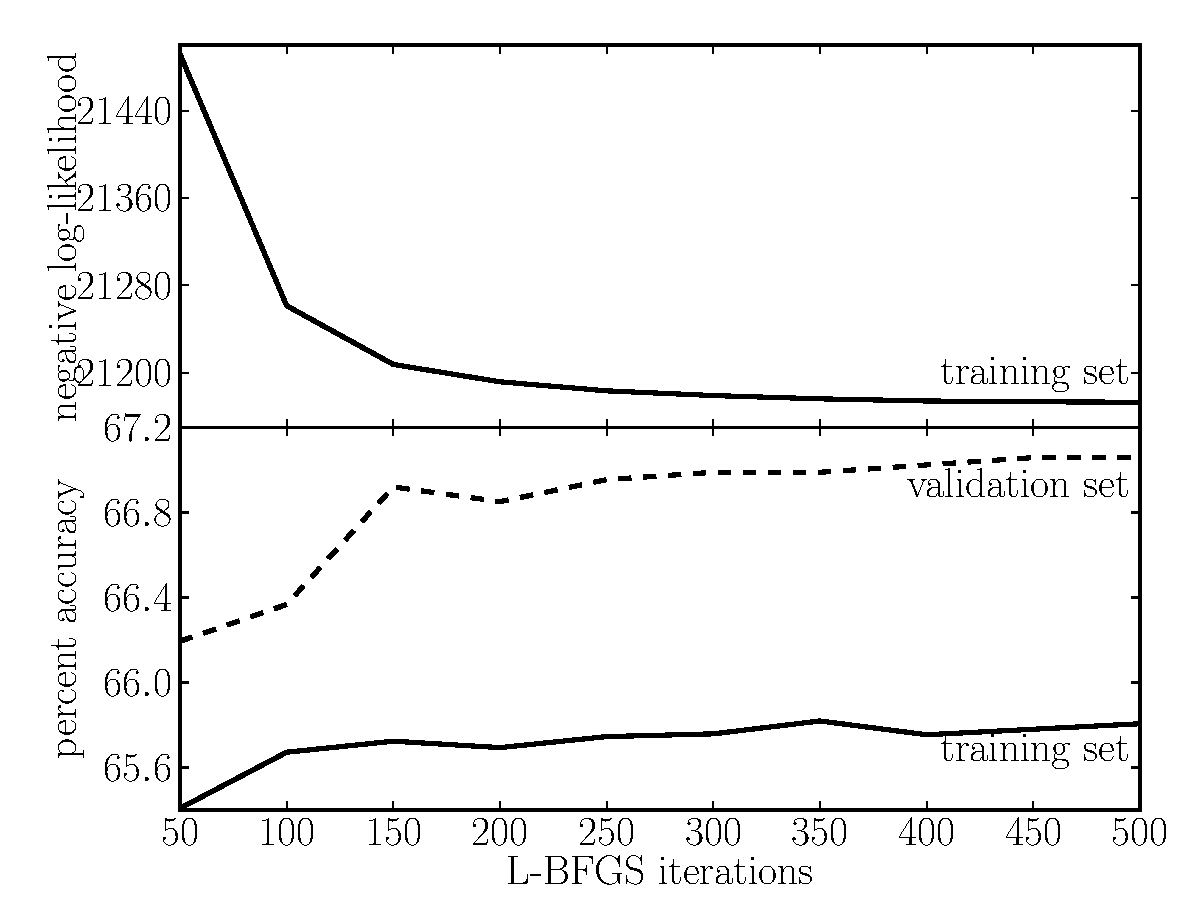
\includegraphics[width=\textwidth]{unigram_convergence.pdf}
\end{center}
\caption{%
The progress of the optimization of equation~\ref{eq:logistic} as a function
of number of iterations.
\emph{top:} The value of equation~\ref{eq:fullmodel}.
\emph{bottom:} The predictive accuracy of the model on the validation and test
sets (as labeled).
\figlabel{unigram-convergence}}
\end{figure}

\begin{figure}[htbp]
\begin{center}
    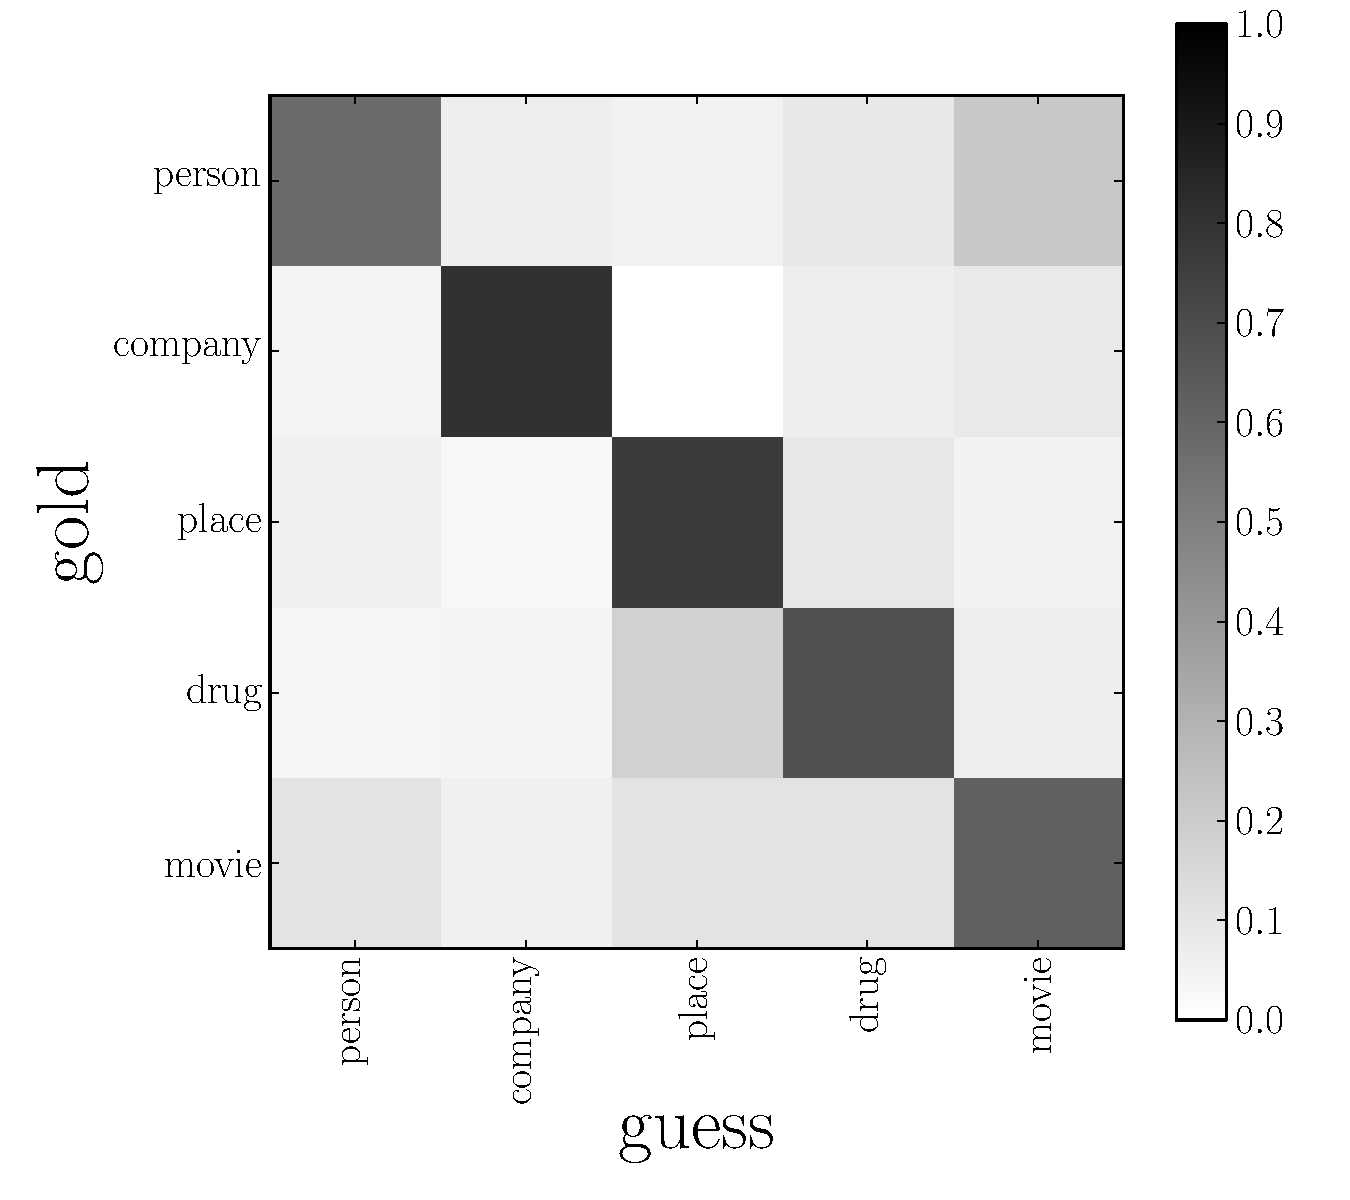
\includegraphics[width=\textwidth]{unigram_confusion.pdf}
\end{center}
\caption{%
The confusion matrix resulting from training $\bvec{W}$ in
equation~\ref{eq:fullmodel} using only unigram features of the training set
and then predicting the validation labels.
\figlabel{unigram-confusion}}
\end{figure}

\begin{figure}[htbp]
\begin{center}
    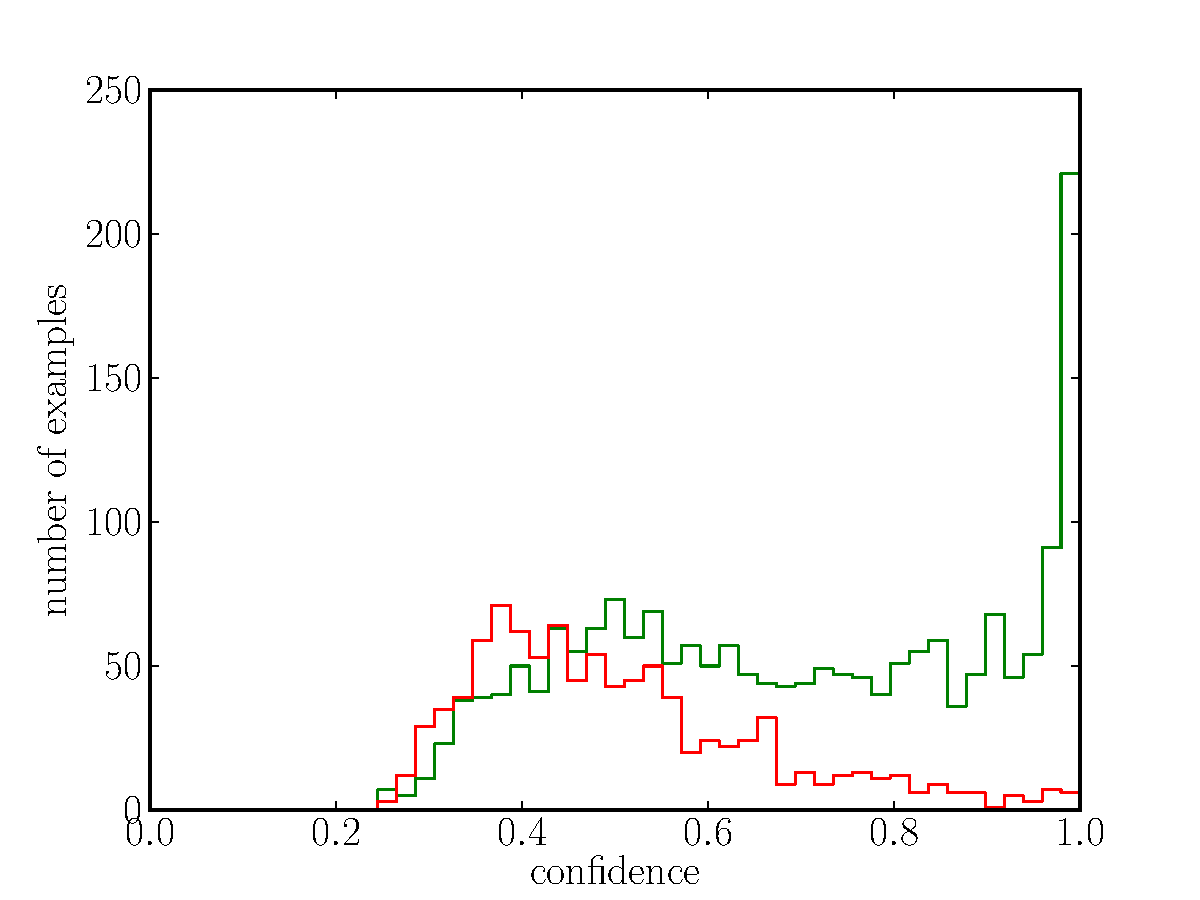
\includegraphics[width=0.7\textwidth]{unigram_confidence_hist.pdf}
\end{center}
\caption{%
\figlabel{unigram-confidence-hist}}
\end{figure}

\begin{figure}[htbp]
\begin{center}
    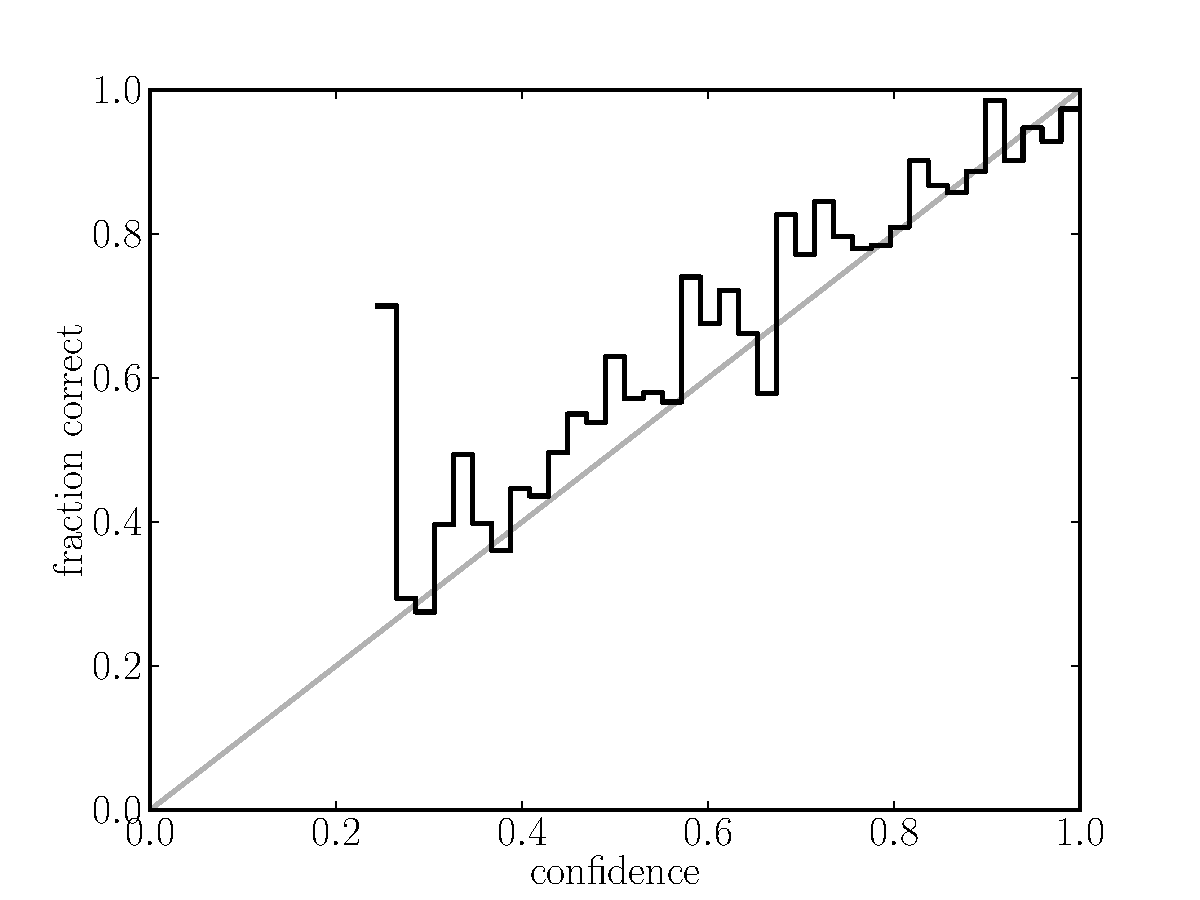
\includegraphics[width=0.7\textwidth]{unigram_confidence_scale.pdf}
\end{center}
\caption{%
\figlabel{unigram-confidence-scale}}
\end{figure}

\section{Larger N-gram models}

\end{document}
